\section{Federated Learning}
\subsection{Concept and Motivation}
\label{subsec:fl_concept}
 
Federated learning (FL) is a distributed machine learning paradigm in which
a model is trained collaboratively across multiple independent nodes without
any raw data leaving its source institution~\cite{mcmahan2017}. Rather than
centralizing training samples on a shared server, FL brings the computation
to the data: each participating node trains a local model on its private
dataset and shares only the resulting model parameters with a central
aggregation server, which combines the updates into an improved global model.
This cycle repeats for a defined number of communication rounds until the
global model converges.
 
The motivation for adopting FL in this work is rooted in the fundamental
tension between data-driven model development and patient privacy. Healthcare
institutions collect large volumes of annotated medical images, yet regulatory
frameworks --- including the Health Insurance Portability and Accountability Act
(HIPAA) in the United States and the General Data Protection Regulation (GDPR)
in the European Union --- impose strict constraints on cross-institutional data
sharing. Negotiating data transfer agreements is costly, time-consuming, and
in many cases legally impractical. FL resolves this tension by enabling
institutions to contribute to a shared model without relinquishing data
custody, making large-scale collaborative medical AI both legally feasible
and technically practical.
 
% -----------------------------------------------------------------------------
\subsection{Federated Learning in Medical Imaging}
\label{subsec:fl_medical}
 
The adoption of FL in the medical domain has grown substantially since its
introduction, driven by the recognition that many clinical datasets are too
small at any single institution to train robust deep learning models, while
the combined data across institutions would be sufficient~\cite{sheller2019}.
FL directly addresses this data insufficiency problem without requiring
physical data consolidation.
 
In medical imaging specifically, FL has been applied across a broad range of
modalities and anatomical targets. Early work by Sheller~\textit{et al.}
demonstrated FL for brain tumor segmentation from MRI scans across multiple
institutions, achieving performance comparable to centralized training without
sharing any patient data~\cite{sheller2019}. Subsequent studies have extended
FL to chest radiograph classification, diabetic retinopathy screening from
fundus photography, histopathology slide analysis, and cardiac structure
segmentation from echocardiography, among others~\cite{rieke2020}.
 
This breadth of applicability is a key motivation for the design of the
proposed system. Rather than building a solution tied to a specific model
architecture or anatomical region, the FL framework developed in this work
is designed to be \textbf{model-agnostic} and \textbf{organ-agnostic}: any
classification or segmentation backbone can be substituted as the local
model, and the training data can comprise images from any body region or
imaging modality. The federated coordination layer — covering client
management, weight aggregation, and communication — remains unchanged
regardless of the underlying clinical task.
 
% -----------------------------------------------------------------------------
\subsection{The Federated Averaging Algorithm}
\label{subsec:fedavg}
 
The aggregation algorithm that underpins the proposed system is Federated
Averaging (FedAvg), introduced by McMahan~\textit{et al.}~\cite{mcmahan2017}
and the most widely adopted FL optimization method to date. FedAvg operates
in iterative communication rounds. Let $K$ denote the number of participating
clients, $\mathcal{D}_k$ the private dataset of client $k$, $n_k =
|\mathcal{D}_k|$ its size, and $n = \sum_{k=1}^{K} n_k$ the total number of
training samples across all clients. The global model at round $t$ is
parameterized by weight vector $\mathbf{w}_t$. Each round consists of three
phases:
 
\textbf{(1) Broadcast.} The server distributes the current global model
weights to all $K$ clients:
\begin{equation}
    \mathbf{w}_t \;\longrightarrow\; \{\text{client}_1, \dots, \text{client}_K\}.
\end{equation}
\textbf{(2) Local Training.} Each client $k$ independently minimizes its
local empirical risk $\mathcal{L}_k$ over $E$ local epochs using a gradient-
based optimizer, producing updated local weights:
\begin{equation}
    \mathbf{w}_t^k \;=\; \mathbf{w}_t \;-\; \eta\,\nabla\mathcal{L}_k(\mathbf{w}_t),
\end{equation}
where $\eta$ is the local learning rate and $\mathcal{L}_k$ is the
task-specific loss function evaluated over the client's local dataset:
\begin{equation}
    \mathcal{L}_k(\mathbf{w}) \;=\;
    \frac{1}{n_k}\sum_{(x_i,\,y_i)\,\in\,\mathcal{D}_k}
    \ell\!\left(f_{\mathbf{w}}(x_i),\,y_i\right).
\end{equation}
 
\textbf{(3) Aggregation.} The server collects the locally updated weights
from all clients and computes the new global model as a weighted average
proportional to each client's dataset size:
\begin{equation}
    \mathbf{w}_{t+1} \;=\; \sum_{k=1}^{K}\frac{n_k}{n}\,\mathbf{w}_t^k.
    \label{eq:fedavg}
\end{equation}
This process minimizes the global objective:
\begin{equation}
    F(\mathbf{w}) \;=\; \sum_{k=1}^{K}\frac{n_k}{n}\,\mathcal{L}_k(\mathbf{w}).
\end{equation}
Equation~\eqref{eq:fedavg} assigns greater influence to clients with larger
datasets, which is appropriate in the medical setting where institutional
dataset sizes vary considerably. Clients contributing more annotated images
should exert proportionally greater influence on the global model.
 
% -----------------------------------------------------------------------------
\subsection{Key Parameters of a Federated Learning System}
\label{subsec:fl_parameters}
 
Configuring a federated learning system involves a distinct set of
parameters beyond those of conventional deep learning. These parameters
govern the coordination between server and clients and directly affect
convergence speed, model quality, communication cost, and privacy. A clear
understanding of each parameter is essential for adapting the system to
different clinical tasks. Table~\ref{tab:fl_params} provides an overview
of the critical parameters and their implications.
 
\begin{table}[!htbp]
\centering
\caption{Key Federated Learning Parameters and Their Clinical Implications}
\label{tab:fl_params}
\begin{tabular}{|p{3.2cm}|p{4.2cm}|p{5.8cm}|}
\hline
\textbf{Parameter} & \textbf{Definition} & \textbf{Implication} \\
\hline
Number of clients ($K$)
    & Total participating institutions
    & More clients improve data diversity and model generalization but
      increase coordination overhead. \\
\hline
Communication rounds ($T$)
    & Number of server--client training cycles
    & More rounds improve accuracy at the cost of higher communication
      volume. Convergence is typically monitored to select $T$. \\
\hline
Client fraction ($C$)
    & Proportion of clients selected per round ($C \in (0,1]$)
    & $C = 1.0$ uses all clients every round (synchronous FL).
      $C < 1.0$ enables asynchronous, scalable training. \\
\hline
Local epochs ($E$)
    & Training epochs each client performs before returning weights
    & Higher $E$ reduces communication rounds but risks \textit{client drift}
      — divergence of local models due to non-IID data~\cite{li2020}. \\
\hline
Local batch size ($B$)
    & Mini-batch size for local gradient computation
    & Affects local convergence speed, memory footprint, and gradient
      privacy (smaller batches increase reconstruction attack risk). \\
\hline
Local learning rate ($\eta$)
    & Step size for local gradient updates
    & Must be tuned per model architecture; too large a value exacerbates
      client drift in non-IID settings. \\
\hline
Aggregation strategy
    & Algorithm used to combine client updates (e.g., FedAvg, FedProx,
      FedNova)
    & Choice depends on data heterogeneity; FedAvg is the standard baseline;
      FedProx adds a proximal term to limit client drift. \\
\hline
Data partitioning scheme
    & How training data is divided across clients (IID vs. non-IID)
    & Non-IID partitions (realistic in healthcare) slow convergence and
      reduce final accuracy compared to IID partitions. \\
\hline
Minimum clients for aggregation
    & Minimum number of client updates required before the server aggregates
    & Prevents the global model from being updated on insufficient
      information; critical for stability. \\
\hline
\end{tabular}
\end{table}
 
Among these, the number of local epochs $E$ and the aggregation strategy
warrant particular attention in the medical imaging context. Increasing $E$
reduces the number of costly communication rounds, which is beneficial in
healthcare networks where bandwidth and uptime may be limited. However,
when client datasets are statistically heterogeneous — a common condition
across hospitals using different scanners, populations, or labeling protocols
— high $E$ causes the local models to overfit to their local distributions
and diverge from the global optimum, a phenomenon known as \textit{client
drift}~\cite{li2020}. The selection of $E$ therefore requires careful
empirical tuning for each deployment scenario.
 
% -----------------------------------------------------------------------------
\subsection{System Architecture Overview}
\subsubsection{Client--Server Design}

The system follows a two-tier federated learning architecture implemented using the Flower (\texttt{flwr}) framework. A single Federated Learning (FL) Server process hosts both the Flower gRPC server and a FastAPI-based REST management API within the same Python process. The Flower server operates on port \texttt{50051}, while the REST management layer operates on port \texttt{8001}. Both services share a common \texttt{SharedState} singleton object that stores the current round status, active model type, round identifier, and the reference to the active Flower thread. This co-location eliminates additional network overhead between the aggregation engine and the management layer and enables efficient coordination between both services.

Each participating hospital deploys an FL Client as a Docker container. Upon startup, the client continuously polls the server's health endpoint until a federated learning round becomes active. Once the server signals round activation, the client initializes the appropriate model according to the task being executed. For any task a client model is instantiated. The client subsequently waits for the gRPC service to become available before connecting through Flower's \texttt{NumPyClient} interface.

A key design principle of the architecture is data locality. Medical images and patient records remain exclusively within the hospital infrastructure and are never transmitted to the central server. Instead, only serialized NumPy arrays containing model parameters are exchanged during federated learning rounds. This design significantly reduces privacy risks while maintaining collaborative model training across institutions.

\begin{figure}[H]
	\centering
	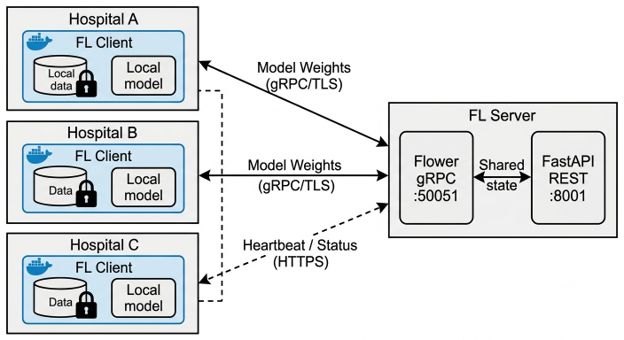
\includegraphics[width=0.9\textwidth]{assets/fl_system_architecture.png}
	\caption{Two-tier federated learning system architecture. Hospital clients communicate with the central federated learning server through TLS-secured gRPC channels, while the REST management layer provides round lifecycle management and monitoring. Raw medical data remains within each hospital boundary.}
	\label{fig:fl_system_architecture}
\end{figure}

\subsubsection{Communication Protocol}

All model parameter exchanges between federated learning clients and the central server are performed using gRPC, Google's high-performance remote procedure call framework built on HTTP/2 and Protocol Buffers. The Flower framework serializes model weight tensors into Protocol Buffer messages before transmission, providing an efficient and platform-independent communication mechanism.

To ensure secure communication, the production deployment uses Transport Layer Security (TLS). Before any model parameters are exchanged, a complete TLS handshake is performed involving a trusted Certificate Authority (CA) certificate, a server certificate, and the server's private key. This process guarantees encrypted communication channels and prevents unauthorized interception or modification of model updates during transmission.

In addition to the gRPC communication channel, the system incorporates a secondary REST-based heartbeat mechanism. Each client periodically sends status reports to the FastAPI management API at a configurable interval, with a default period of 15 seconds. These heartbeat messages include metadata such as the currently active model type and the active federated learning round identifier.

The heartbeat channel provides real-time visibility into client participation and system health while maintaining patient privacy. No medical images, patient records, or other sensitive clinical information are transmitted through this channel. Instead, it serves exclusively for monitoring, synchronization, and lifecycle management purposes.

The server broadcasts the active model type to all clients before the start of each federated learning round. This ensures that all participating institutions instantiate and train identical model architectures, thereby maintaining consistency during the aggregation process.

\subsection{Model Architecture}
\subsubsection{Federated Learning Workflow}

Federated Learning (FL) is a distributed machine learning paradigm that enables multiple clients to collaboratively train a shared global model without directly exchanging their local data. Instead of transferring datasets to a centralized location, each client performs training locally and only shares model updates with a coordinating server. This approach preserves data privacy while allowing the model to benefit from knowledge learned across multiple data sources.

The federated learning process proceeds iteratively through a sequence of communication rounds. At the beginning of each round, the central server distributes the current global model to participating clients. Each client then trains the model on its local dataset and computes updated model parameters. These parameters are subsequently transmitted back to the server, where they are aggregated to produce a new global model.

This collaborative training framework offers several advantages, including improved privacy, reduced data-sharing requirements, and the ability to leverage geographically distributed datasets. As a result, federated learning has become an attractive solution in domains where data governance, confidentiality, or regulatory constraints limit centralized data collection.

\subsubsection{Local Data Processing}

Prior to local training, each client performs preprocessing on its own dataset according to a predefined and consistent pipeline. Standardized preprocessing ensures that data representations remain compatible across clients and that model updates are learned under similar conditions.

Typical preprocessing operations may include:

\begin{itemize}
	\item Data cleaning and quality control
	\item Feature normalization or standardization
	\item Input resizing or formatting when required
	\item Training-time augmentation or transformation strategies
\end{itemize}

During validation and evaluation, only deterministic preprocessing operations are applied to ensure that performance metrics accurately reflect the model's generalization capability.

By maintaining a consistent preprocessing procedure across all participating clients, federated learning systems reduce variability introduced by differences in local data sources and collection procedures.

\subsubsection{Local Training and Model Updates}

Each participating client receives the current global model from the federated server and performs training on its local dataset for a predefined number of epochs or optimization steps. The training process follows the same objective function and optimization strategy across all clients to ensure consistency during aggregation.

After local training is completed, the client generates a set of updated model parameters representing knowledge learned from its local data. Rather than transmitting raw data samples, only these model updates are communicated to the federated server.

The use of local training provides several benefits:

\begin{itemize}
	\item Data remains within the client environment.
	\item Communication involves model parameters rather than datasets.
	\item Learning can exploit knowledge from diverse and distributed data sources.
	\item Privacy risks associated with centralized data storage are reduced.
\end{itemize}

\subsubsection{Global Aggregation}

Upon receiving updates from participating clients, the federated server combines the local model parameters to produce an improved global model. The most common aggregation strategy is Federated Averaging (FedAvg), where client updates are weighted according to the amount of local training data available at each client.

The aggregation process can be expressed as:

\[
w^{(t+1)} = \sum_{k=1}^{K} \frac{n_k}{N} w_k^{(t)},
\]

where:

\begin{itemize}
	\item $w^{(t+1)}$ denotes the updated global model parameters,
	\item $w_k^{(t)}$ represents the parameters received from client $k$,
	\item $n_k$ is the number of training samples at client $k$,
	\item $N = \sum_{k=1}^{K} n_k$ is the total number of samples across all participating clients,
	\item $K$ is the number of participating clients.
\end{itemize}

After aggregation, the updated global model is redistributed to clients, and the next communication round begins. Through repeated rounds of local training and global aggregation, the model gradually converges toward a solution that reflects information learned from all participating clients.

\subsubsection{Model Evaluation and Checkpointing}

To monitor training progress and ensure model quality, each client performs validation using a local validation dataset. Evaluation metrics are computed after training intervals and can be used to assess convergence and generalization performance.

A common practice is to employ best-model checkpointing, where the model parameters corresponding to the best validation performance are preserved during local training. At the conclusion of a training round, the selected parameters are used to generate the client update transmitted to the federated server.

This strategy helps prevent the propagation of overfitted local models and improves the overall stability and generalization of the aggregated global model. By combining locally optimized updates from multiple participants, federated learning achieves collaborative model improvement while maintaining data locality and privacy.

\subsection{Privacy and Security}

\subsubsection{Core Privacy Guarantee}

The primary privacy advantage of federated learning is that raw patient data never leaves the originating healthcare institution. Medical images, metadata, and associated clinical records remain stored locally, while only model parameters are exchanged during training.

Compared to centralized machine learning approaches, this architecture substantially reduces the risk associated with large-scale data breaches and simplifies compliance with healthcare regulations such as HIPAA and GDPR.

Only model weight tensors are transmitted between clients and the central server, ensuring that explicit patient identifiers are never exposed during the learning process.

\subsubsection{Centralized vs. Federated Comparison}

Table~\ref{tab:centralized_federated} summarizes the major privacy and security differences between centralized and federated learning approaches.

\begin{table}[H]
	\centering
	\caption{Privacy and Security Comparison Between Centralized and Federated Learning}
	\label{tab:centralized_federated}
	\begin{tabular}{|l|c|c|}
		\hline
		\textbf{Property} & \textbf{Centralized} & \textbf{Federated} \\
		\hline
		Raw data leaves institution & Yes & No \\
		Single point of data breach & Yes & No \\
		HIPAA/GDPR compliance & Difficult & Easier \\
		Shared artifact & Full dataset & Model weights only \\
		Supports differential privacy & N/A & Yes \\
		Resilient to server breach & No & Partial \\
		\hline
	\end{tabular}
\end{table}

Federated learning eliminates the need for centralized storage of medical imaging datasets, thereby reducing regulatory burden and minimizing exposure of sensitive patient information.

\subsubsection{Known Threats and Mitigations}

Although federated learning significantly improves privacy, it does not completely eliminate all attack vectors. Several threats remain relevant, particularly those attempting to reconstruct information from shared model updates.

The system incorporates multiple mitigation mechanisms designed to reduce the effectiveness of such attacks while preserving model utility.

\subsubsection{Gradient Inversion Attacks}

Gradient inversion attacks attempt to reconstruct training samples from model updates shared during federated learning.

An adversary with access to model gradients may iteratively optimize synthetic inputs until their gradients resemble the observed updates, potentially revealing information about the original training data.

The effectiveness of these attacks decreases substantially as batch size increases because gradients become aggregated across multiple samples.

The system therefore enforces minimum batch sizes:

\begin{itemize}
	\item DenseNet-121: $B \ge 32$
	\item YOLOv8n (CPU): $B \ge 8$
	\item YOLOv8n (GPU): $B \ge 16$
\end{itemize}

These constraints reduce the feasibility of reconstructing individual patient images from shared updates.

\subsubsection{Differential Privacy}

For deployments requiring stronger privacy guarantees, the architecture supports Differential Privacy (DP) through Gaussian perturbation of model updates before transmission.

The private update rule is defined as:

\[
\tilde{w}_{k}^{t}
=
w_{k}^{t}
+
\mathcal{N}
\left(
0,\,
\sigma^{2}C^{2}I
\right)
\]

where:

\begin{itemize}
	\item $w_k^t$ is the original model update,
	\item $C$ is the clipping threshold,
	\item $\sigma$ is the noise multiplier,
	\item $\epsilon$ represents the privacy budget,
	\item $\delta$ represents the failure probability.
\end{itemize}

\begin{figure}[H]
	\centering
	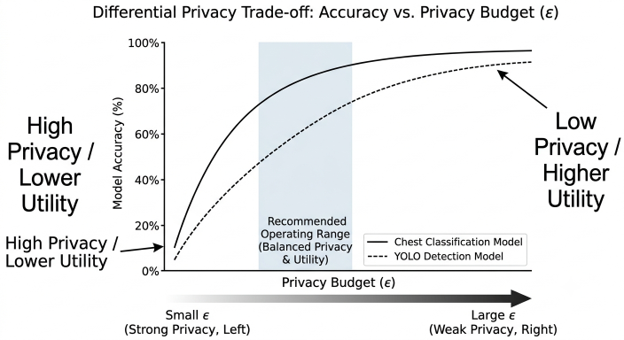
\includegraphics[width=0.8\textwidth]{assets/privacy_utility_tradeoff.png}
	\caption{Privacy--utility tradeoff under $(\epsilon,\delta)$-differential privacy. Smaller values of $\epsilon$ provide stronger privacy guarantees but may reduce model performance.}
	\label{fig:dp_tradeoff}
\end{figure}

\subsubsection{Additional Privacy Considerations}

Beyond gradient inversion attacks, model inversion and membership inference attacks represent additional privacy concerns.

Model inversion attempts to reconstruct representative training samples from a trained model, while membership inference seeks to determine whether a specific record was used during training.

Federated aggregation, large batch sizes, and differential privacy collectively reduce the effectiveness of these attack vectors.

\subsubsection{Transport-Layer Security (TLS)}

All model parameter exchanges are protected using mutual Transport Layer Security (mTLS) over gRPC.

The security infrastructure consists of:

\begin{itemize}
	\item Certificate Authority certificate (\texttt{ca.crt})
	\item Server certificate (\texttt{server.pem})
	\item Server private key (\texttt{server.key})
\end{itemize}

Mutual authentication ensures confidentiality, integrity, server authentication, and client authentication during communication.

In production deployments, TLS is mandatory and protects all federated learning traffic against interception and tampering.

\subsubsection{Authentication and Access Control}

Each participating institution receives a unique client identifier and API key during enrollment.

These credentials are required before client startup and are validated for every REST API request.

The authentication framework ensures:

\begin{itemize}
	\item Only authorized hospitals can participate.
	\item Unauthorized clients cannot submit updates.
	\item Client activity can be audited through server logs.
	\item Credentials remain external to source code repositories.
\end{itemize}

\subsubsection{Round Integrity and Liveness Controls}

The system continuously verifies round status before and during local training.

If a round is cancelled or completed, participating clients immediately terminate local computation and prevent obsolete updates from reaching the aggregation server.

Heartbeat messages are transmitted every fifteen seconds, enabling real-time monitoring of client availability and participation status.

These mechanisms improve both system integrity and operational reliability.

\subsubsection{Security Implementation Status Summary}

Table~\ref{tab:security_controls} summarizes the implementation status of all security controls incorporated into the federated learning platform.

\begin{table}[H]
	\centering
	\caption{Security Controls -- Implementation Status}
	\label{tab:security_controls}
	\renewcommand{\arraystretch}{1.2}
	\begin{tabularx}{\textwidth}{|p{3.8cm}|p{2cm}|p{1.8cm}|X|}
		\hline
		\textbf{Security Control} &
		\textbf{Category} &
		\textbf{Status} &
		\textbf{Notes} \\
		\hline
		
		Data locality (no raw data transmitted) &
		Privacy &
		Done &
		Core FL design property; only weight tensors transmitted \\
		\hline
		
		TLS encryption on gRPC channel &
		Transport &
		Done &
		\texttt{ca.crt} + \texttt{server.pem} + \texttt{server.key}; mutual TLS \\
		\hline
		
		API key authentication &
		Access Control &
		Done &
		\texttt{CLIENT\_API\_KEY} required; validated on every REST call \\
		\hline
		
		Client identity validation &
		Access Control &
		Done &
		\texttt{CLIENT\_ID} required; startup exit if absent \\
		\hline
		
		Large batch size ($B \geq 32$) &
		Privacy &
		Done &
		Mitigates gradient inversion attack fidelity \\
		\hline
		
		Heartbeat liveness monitoring &
		Integrity &
		Done &
		Continuous per-client liveness signal every 15 seconds \\
		\hline
		
		Per-epoch round-active check &
		Integrity &
		Done &
		Aborts training on cancelled round; covers both model types \\
		\hline
		
		Best-model checkpoint (local) &
		Robustness &
		Done &
		Restores best validation-loss weights before uploading to server \\
		\hline
		
		Selective YOLO federation (no head) &
		Integrity &
		Done &
		\texttt{cv3} detection head excluded from aggregation to prevent shape mismatch \\
		\hline
		
		Differential Privacy (DP noise) &
		Privacy &
		CONFIG-URABLE &
		Architecture supports $(\epsilon,\delta)$-DP; not yet enabled by default \\
		\hline
		
		Secure credential storage &
		Access Control &
		Done &
		\texttt{.env.template} pattern; credentials never stored in source code or container images \\
		\hline
		
		Shutdown-on-breach notification &
		Resilience &
		Done &
		Server sends \texttt{round-failed} webhook on unexpected shutdown \\
		\hline
		
	\end{tabularx}
\end{table}

The current implementation includes fully operational transport security, authentication, access control, liveness monitoring, and round integrity mechanisms. Differential privacy remains available as a configurable enhancement for deployments requiring stronger formal privacy guarantees.
\subsection{What Makes the Proposed System Distinctive}
\label{subsec:fl_novelty}
 
While federated learning has been applied in various medical imaging studies,
the majority of existing implementations are designed around a fixed model
architecture and a specific anatomical target, limiting their transferability
to new clinical tasks. The proposed framework differentiates itself through
the following design principles:
 
\textbf{Model Agnosticism.} The federated coordination layer — encompassing
client management, weight serialization, aggregation, and communication — is
fully decoupled from the local model definition. Any differentiable model
that can be expressed as a parameter vector (e.g., CNNs for classification,
U-Net variants for segmentation, Vision Transformers) can be substituted as
the local model without modifying the federated infrastructure. This makes
the system immediately applicable to new imaging tasks simply by swapping the
model definition on the client side.
  
\textbf{Staged Data Integration.} The system incorporates a staged data
feeding protocol that progressively increases each client's active training
subset across federated rounds. This design reflects the clinical reality
that expert-annotated medical imaging datasets grow incrementally over time
as radiologists label new cases. Rather than requiring a fully annotated
dataset before training begins, the system accommodates continuous data
growth, enabling earlier model deployment and iterative improvement as
annotation progresses.
 
\textbf{Containerized Reproducibility.} Each participating node is deployed
as an isolated Docker container, ensuring that the federated environment is
fully reproducible across different hardware configurations and operating
systems. The container-based architecture also simplifies scaling: adding a
new institution requires only the deployment of an additional client
container with the appropriate data volume mount, with no changes to the
server or existing clients.
 
\textbf{Framework Choice.} The system is implemented using the Flower
(flwr) framework~\cite{beutel2022}, selected for its support of multiple
ML backends (PyTorch, TensorFlow, JAX), its clean abstraction of the
client-server protocol, and its active development for healthcare FL
research. The backend-agnostic design of Flower further reinforces the
model-agnostic objective of the proposed system.
 
Collectively, these properties position the proposed FL framework as a
general-purpose infrastructure for privacy-preserving collaborative medical
image analysis, extensible to a wide range of clinical specialties and
diagnostic tasks without architectural redesign.
